% !TEX root = ../notes_template.tex
\chapter{Metagenomics}\label{chp:metagenomics}

\minitoc
\section{Introduction to Microbiome}
TO DO: Add One Health Concept Era and improve \autoref{fig:microbes_everywhere}.

Microbes are everywhere, almost every environment on earth is colonized by different types of organisms \autoref{fig:microbes_everywhere}. 

\begin{definition}[Ecosystem]
    An ecosystem is a community or group of organisms that live and interact with each other in a specific environment
\end{definition}
So, microbes do not live isolated but instead live in different and complex ecosystems. We can distinguish three main 
categories of ecosystems: Host-Associated, Environmental, and Engineered.
\begin{itemize}
    \item In the Host-Associated ecosystem the microbes live within a Host, that could be any animal that you think of 
    but also humans, and they can play active roles in pathogen resistance, immune modulations, and food metabolism, among others.
    \item Also we have the environmental category, that includes the marine and soil ecosystems, being involved in carbon 
    sequestration, pathogen resistance, nutrient absorption, and soil fertility.
    \item Finally, we can also classify the ecosystems as engineered all the artificial or human-created ecosystems 
    where microbes can live. This includes the wastewater treatment in activated sludge…etc. They raise special interest 
    in the biotechnology field.
\end{itemize}
\begin{figure}[!ht]
    \centering
    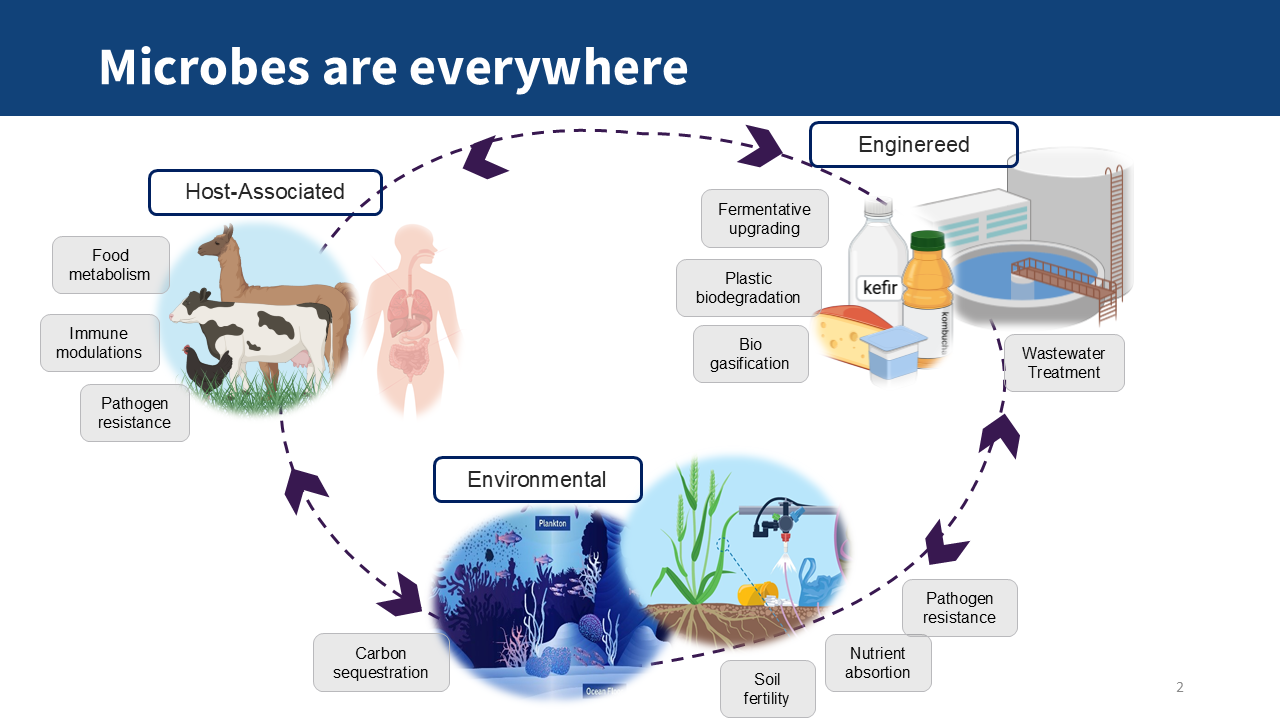
\includegraphics[width=1\linewidth]{./figure/microbes_everywhere.png}
    \caption{One Health concept, microbes are everywhere}
    \label{fig:microbes_everywhere}
\end{figure}

\begin{definition}[Microbiome]
    The words “micro” and “biome” are of Ancient Greek origin. “Micro” ($\mu\iota\kappa\rho o\zeta$) means small, while 
    the term “biome” is composed of the Greek word bíos ($\beta\iota o \zeta$, life) and modified by the ending “ome” (Anglicization of Greek).
\end{definition}
\begin{definition}[Microbiota]
    The words “micro” and “biota” are also of Ancient Greek origin. It is a combination of “Micro” ($\mu\iota\kappa\rho o \zeta$, small), with 
    the term “biota” ($\beta\iota o \tau\alpha$), which means the living organisms of an ecosystem or a particular area.
\end{definition}
\begin{definition}[Microbiome]
    The term microbiome includes both the microbiota (community of microorganisms) and their “theatre of activity”, 
    which includes structural elements such as proteins, lipids and theirs genomes, but also genetic mobile elements such 
    as plasmid, the metabolites produced by the microbes, and the surrounding environmental conditions.
\end{definition}
So, it's important to understand that, in contrast to the microbiota which can be studied separately, for example using a 
petri dish, the microbiome is not only composed of the microorganisms that live within, but also all this other elements 
(“Threatre of activity”) \autoref{fig:microbiome_definition} that directly interact with each other and impact the function 
and type of microbiota present in this ecological niche.

\begin{figure}[!ht]
    \centering
    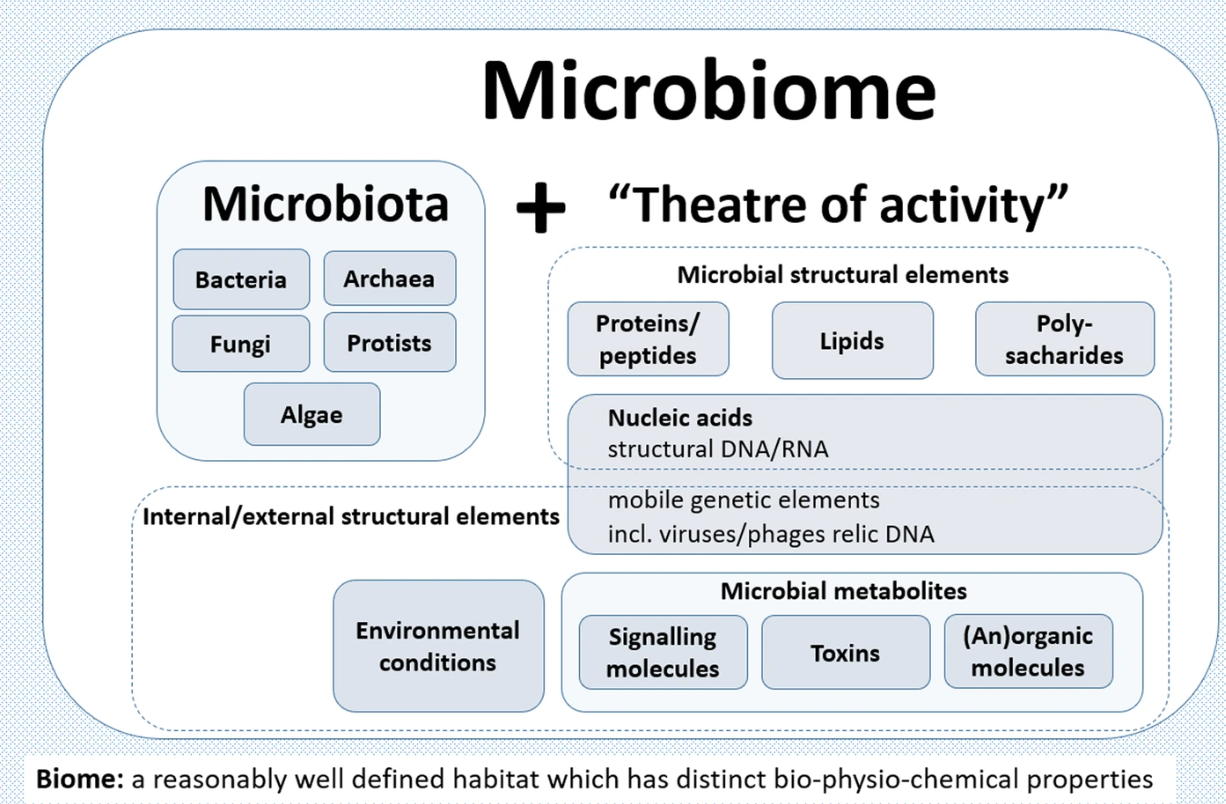
\includegraphics[width=1\linewidth]{./figure/microbiome_definition.png}
    \caption{Borrowed from \citetitle{Berg2020} \cite{Berg2020}}
    \label{fig:microbiome_definition}
\end{figure}

You will see frequently that microbiome studies often focus on one or few specific groups of the microbiota, for example, 
only the bacteria part, using terms such as bacteriome. More unusual they can also focus on archaeome, or mycobiome, 
referring to archaeal and fungal communities, respectively. Lately some studies are also interested in the viral part 
of the microbiome, which can be referred to as virome. But also, they can focus on one of the elements of this 
“threatre of activity”. When we focus on studying the genomes of the microbiome, which are called metagenomes, we are 
doing metagenomics. The same applies for the transcriptome, metatranscriptome - metratranscriptomics; 
metaproteome - metaproteomics; metabolome - metabolomics. Later on we will see some of these topics more in detail.

\section{Taxonomical Classification}
There is also a question of at what resolution each of the microbiome members should be studied. This resolution depends 
on the taxonomic level we are studying the microbiome. There are 9 major taxonomic levels or clades, with its corresponding 
abbreviation, ranging from very general (Domain) to specific (Strain), going to many other clades such as phylum, family or genus. 
There might also be intermediate clades, such as subphylum between phylum and class, and subspecies between species and strain.


Note that according to the International Code of Nomenclature of Prokaryotes, it is recommended to print scientific names 
by a different typeface, e.g., italic, or by some other device to distinguish them from the rest of the text. The name of a 
genus should be spelled without abbreviation the first time it is used. Later use of the name of the species previously cited 
usually has the name of the genus abbreviated, commonly to the first letter of the generic name. 
Example: Clostridioides difficile. -> C. difficile If, however, species are listed belonging to two or more genera which have 
the same initial letter, the generic name should be used in full, or initial two-letter or three-letter abbreviations 
should be used. Some subcommittees on taxonomy have recommended three-letter abbreviations to be used in such cases.


Here we have two samples, one the one side the taxonomic classification of C. difficile, bacteria known to cause diarrheal 
infections, and on the other side L. crispatus, the taxonomic classification of one bacteria commonly found in the vaginal 
microbiome. You can see that for these organisms, all the taxonomic levels are complete, but that's the perfect scenario. 
The reality is that, in 2019, one study showed that 85/119 phyla have not had a single species described to date. So, 
you commonly will find microbes that are only taxonomic classified up to the genus or family level, having subsequent 
unknown clades. For this reason it is important to keep in mind that taxonomical classification is constantly changing.

Also, there might be discrepancies in the classification according to the methodology used to define each clade. 
For prokaryotes, two most widely used are NCBI taxonomy (which is the one actually used to these microbes) and 
GTDB (C. difficile is p\_\_Bacillota\_A). NCBI taxonomy is pretty useful because of its synonyms (example). Worth mentioning 
is the python package (ETE toolkit, v.4.) that allows access programmatically to both databases and retrieve the 
lineage of a desired microbe.



\section{Quality Control}
In this section, we will evaluate critical quality control metrics that are essential for ensuring the integrity and reliability 
of metagenomics datasets. These metrics help assess the overall quality of sequencing data and determine whether any 
technical artifacts or contamination could influence the downstream analysis. Below are the key metrics we will focus on:
\begin{itemize}
    \item[Number of Reads per Sample (in Gigabase Pairs, Gbp)] The number of reads per sample, expressed in Gbp, is a 
    fundamental metric that indicates the amount of sequencing data generated for each sample. Sequencing depth is 
    crucial for accurately detecting microbial species and other biological signals, as deeper sequencing provides a more 
    comprehensive representation of the microbial community. In the plot, we represent three stages of data processing, 
    each with its own Gbp value:
    \begin{itemize}
        \item[Raw Data (Raw)] This represents the total number of reads generated directly from sequencing, before any 
        quality control or filtering.
        \item[After Filtering (Filt)] This value reflects the number of reads retained after applying the tool fastp to 
        remove low-quality sequences, adapters, and other artifacts. Filtering ensures that only high-quality reads are 
        included in the analysis, improving accuracy.
        \item[After Decontamination (Deconta)] This shows the number of reads left after human DNA decontamination, 
        where sequences that map to the human genome are removed. This step is particularly important in metagenomics 
        studies to prevent human DNA contamination from masking microbial signals or skewing results.
    \end{itemize}
    \item[Percentage of Mapped Reads to Human DNA] This metric represents the proportion of reads that align to the human 
    genome. A high percentage indicates significant contamination from human DNA, which is often unavoidable in samples 
    like skin. However, too much human DNA can obscure microbial diversity, making it essential to identify and remove 
    these sequences during the quality control process. Monitoring this metric helps ensure the decontamination step is 
    effective.
    \item[Percentage of Duplication] Duplication percentage refers to the proportion of reads that are duplicates of 
    each other. High duplication rates can indicate over-sequencing or PCR amplification bias, which can distort microbial 
    abundance estimates. Controlling for duplication ensures the data accurately reflects the diversity and relative 
    abundance of species in the sample.
    \item[Percentage GC Content] GC content is the percentage of guanine and cytosine nucleotides in the sequencing reads. 
    This metric provides insight into the overall nucleotide composition of the dataset and can be used to identify 
    potential biases or anomalies. For instance, extreme deviations in GC content might suggest contamination, poor 
    sequencing quality, or species-specific biases in the dataset.
    \item[Percentage Adapter Content] Adapter content refers to the proportion of sequences that still contain adapter 
    sequences from the library preparation process. Adapter contamination can interfere with downstream analysis, so it 
    is critical to ensure that adapters are effectively removed during the filtering process. A low percentage of adapter 
    contamination indicates good-quality data.
    \item[Percentatge of Reads assigned by Taxonomical profiling tool] MetaPhlAn4 is a popular tool used to classify 
    microbial taxa from metagenomic data. This metric shows the percentage of reads that could be assigned to specific 
    taxa using MetaPhlAn4. A high percentage of assigned reads suggests successful identification of microbial species, 
    while a low percentage may indicate poor sequencing quality, high contamination, or the presence of uncharacterized 
    species in the dataset.
\end{itemize}

\section{Microbial Diversity}
The diversity definition according to the Cambridge dictionary is the fact of many different types of things or people being included 
in something. If we translate this term into the microbial context is the fact of many different microbes (or so called 
biological variability) included in something. Depending on this something, we will differentiate between alpha and beta
diversity \autoref{fig:microbial_diversity}.

\begin{figure}[!ht]
    \centering
    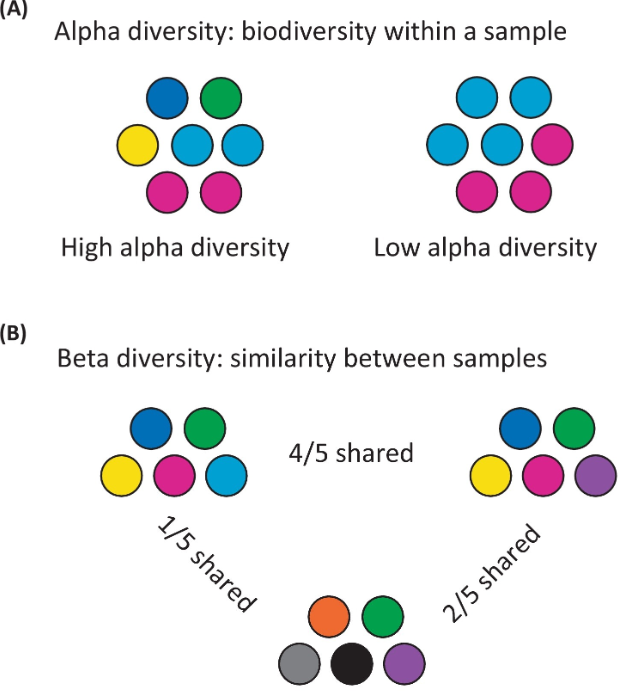
\includegraphics[width=1\linewidth]{./figure/microbial_diversity.png}
    \caption{(A) Alpha diversity represents the biodiversity (species richness) within a specific community or individual 
    sample. The sample on the left has high alpha diversity (five bacterial taxa), while the sample on the right has low 
    alpha diversity (two bacterial taxa). (B) Beta diversity represents how similar one community or individual sample 
    is to another. The samples on the left and right are similar to each other (4/5 shared bacterial taxa), while the 
    sample on the left is not very similar to the sample in the middle (1/5 shared bacterial taxa). 
    Borrowed from \citetitle{Thrackray2019} \cite{Thrackray2019}.}
    \label{fig:microbial_diversity}
\end{figure}


\subsection{Alpha diversity}
Alpha diversity is a way to measure how many different types of microorganisms (species) are present in a sample and how 
evenly distributed they are. There are two main components:
\begin{itemize}
    \item[Species Richness] This refers to the number of different species present in a sample. For example, if you took 
    a sample from the gut, species richness would tell you how many different species of bacteria are there.
    \item[Species Evenness] This indicates how evenly the individuals are distributed among those species. A community 
    where a few species dominate would have low evenness, whereas one where all species have similar abundance would have high evenness.
\end{itemize}

We will measure the two following indexes:
\begin{itemize}
    \item[Chao1 index] is used to estimate species richness, i.e., the total number of different species present in a 
    sample. It is especially useful when the sample has many rare or unobserved species.
    \item[The Shannon index (or Shannon-Weaver index)] measures both species richness and evenness, i.e., how evenly the 
    individuals are distributed among the different species in the sample. Chao1 is often used when there is concern about 
    underestimating the true number of species due to sampling limitations, whereas Shannon is used to assess the overall 
    diversity structure of a community, considering both richness and evenness cause is weighted by richness.
    \item[Simpson] Distribution evenly taxa (evenness). Weighted by richness.
    \item[ACE]
    \item[FaithPD] phylogenetic relatedness between taxa.
\end{itemize}


\section{Metagenomes reconstruction}
\subsection{Assembly}

Metagenomic assembly challenges that complicate the assembly and fragmenting of contigs:
\begin{itemize}
    \item Highly non-uniform read coverage across different genomes. Widely different abundance levels of various species 
        within a microbial sample.
    \item Shared conserved genomic regions across species, so call 'interspecies repeats'. They migh trigger intergenomic 
        assembly errors.
    \item Closely related bacterial strains representing a bacterial species. Many bacterial species in a microbial sample 
        are represented by \textit{strain mitxures}, which are multiple related strain with varying abundances.
    \item High microbial diversity of certain enviroments. Comparison soil samples vs vaginal microbiome.
\end{itemize}

\subsubsection{metaSPAdes}
metaSPAdes is a state-of-the-art tool for assembling metagenomic sequencing data, addressing the challenges of mixed and 
complex microbial communities.

\begin{enumerate}
    \item Sequence fragmentation into k-mers.
    \item Error correction by k-mer abundance analysis.
    \item Multisized de Bruijn graph construction with k-mers of different length.
    \item Bulge corremoval by removing edged from bulger and recording its information for later use.
    \item Detection and masking of strain variation. To respond the the microbial diversity challenge, metaSPAdes focuses on 
    reconstructing a consensus backcone of a strain mixture, ignoring some strain-specific features corresponding to rare strains.
    \item Iterative graph refinement.
    \item Output Contigs by reconstruction paths in the assembly graph.
\end{enumerate}


\textbf{Sequence fragmentation}. Input sequencing reads (e.g. paired-end reads of 150 bp, PE150) are split into smaller 
overlapping pieces called k-mers. These k-mers, substrings of fixed length \textit{k}), will represent the building blocks for
the subsequent graph construction. K-mers allow efficent handling of overlapping sequences, enabling the identification of 
how reads connect to from longer genomic fragments. For example: Read = ACGTAGC; k=3 $\arrowvert$ k-mers: ACG, CGT, GTA, TAG, AGC.

\textbf{Error correction}. Errors in sequencing (e.g., substitutions, insertions) create false k-mers that don't actually 
belong to the genome. MetaSPAdes uses the abundance of each k-mer to detect and correct these errors. High-abundance k-mers 
are more likely to be real, whereas low-abundant k-meres are considered likely errors and are corrected or removed. Removing 
errors reduces the graph's complexity, making the assembly more accurate and faster. If a sequencing error changes a k-mer 
ATCG to ATCC, and ATCC is detected in only one read, it can be corrected back to ATCG if supported by other reads.

\textbf{Multisized de Bruijn graph construction}. With our k-mers we will construct the alignment using a de Bruijn 
graph, where is node represents a k-mer and overlap between the k-mers are represented by an "arrow" (called directed edge).
However, the choice of k affects the construction of the de Bruijn graph. Smaller values of 
k collapse more repeats together, making the graph more tangled. Larger values of k may fail to detect overlaps between 
reads, particularly in low coverage regions, making the graph more fragmented. Since low coverage regions are typical for 
SCS data, the choice of k greatly affects the quality of single-cell assembly. Ideally, one should use smaller values of 
k in low-coverage regions (to reduce fragmentation) and larger values of k in high-coverage regions (to reduce repeat 
collapsing). Therefore metaSPAdes constructs multiple de Bruijn graphs using different k values, and combined them into 
a \textbf{multisized de Bruijn graph}, balacing resolution and connectivity. 
SPAdes is a universal A-Bruijn assembler in the sense that it uses k-mers only for building the initial de Bruijn graph 
and "forgets" about them afterwards; on subsequent stages it only performs graph-theoretical operations on graphs that 
need not be labeled by k-mers. The operations are based on graph topology, coverage, and sequence lengths, but not the 
sequences themselves. At the last stage, the consensus DNA sequence is restored. Example: Bacteria A has many reads, so it 
forms a dense graph with many overlapping k-mers. Bacteria B and C have fewer reads, making their graphs sparser but 
still detectable due to combined k-mer sizes.


\textbf{Bulge corremoval}. Existing assembers often use two complementary approaches to deal with errors 
in reads: (1) error correction in reads and (2) \gls{bulge}/bubble removal in de Bruijn graphs. Note the surprising contrast 
between these two approaches, both aimed at the same goal: the former approach corrects rather than removes erroneous 
k-mers in reads, while the latter approach removes rather than corrects erroneous k-mers in de Bruijn graphs. 
Removal (rather than correction) of bulges leads to deterioration of assemblies, since important information (particularly 
in the case of SCS) may be lost. SPAdes, unlike other NGS assemblers, records information about removed edges from 
bulges for later use before discarding them. We thus call this procedure "bulge correction and removal" (or bulge corremoval).
SPAdes maintains a data structure allowing one to backtrack all bulge corremovals. This is used in later stages of SPAdes 
to map reads to the assembly graph.

\textbf{Decting and masking strain variation}. Aiming at the consensus assembly of a strain mixture, metaSPAdes masks the 
majority of strain differences using a modification of the SPAdes procedures for masking sequencing errors. Genomic differences 
caused by sequecing errors often result in "bulges" and "tips" in the de Bruijn graphs. For example, an artifact often 
results in a bulge formed by two short alternative paths between the same vertices in the de Bruijn graph, a "correct" 
path with high coverage and an "erroneous" path with low coverage. Similarly, a substitution or a small indel in a rare 
strain (compared with an abundant strain) often results ina buldge formed by a high-coverage path corresponding to the 
abundant strain and an alternative low-coverage path corresponding to the rare strain.

\textbf{Iterative graph refinement}. The graph undergoes multiple rounds of refinement. (1) Ambigous regions are clarified,
(2) Information from different k-mer sizes is combined, (3) remaining spurious connections are removed,

\textbf{Output Contigs}. Paths in the assembly graph are reconstructed into long sequences (contigs). This involves tracing 
through the graph to identify sequences that correspond to genomic fragments. Long, continuous sequences representing reconstructed 
portions of the genomes. Well-covered regions produce high-quality contigs, while low-coverage or ambiguous regions may 
remain fragmented.

\subsubsection{MEGAHIT}


\subsection{Binning}
Binning. Critical step required to establish a genome from a metagenomic assembly. This involves assignment of assembled 
fragments to a draft genome based on detection on any scaffold of some signal(s) that occur(s) locally within a genome and 
persists genome-wide \cite{Chen2020}. 

Genome curation \cite{Hiltemann2023,microbiome-metagenomics-binning}. Filling scaffolding gaps and removal of local assembly 
errors. Gap filling strategies: 
\begin{itemize}
    \item[GapFiller] Tool for filling the N's gaps at scaffold joins. Often a few iterations are needed for gap closure. Using:
    \begin{itemize}
        \item Unplaced pairs for reads adjacent to the gaps. When reads are mapped to genome fragments that compose a bin, a 
        file of unplaced paired reads is generated for each fragment.
        \begin{itemize}
            \item If due to low coverage gap filling is not achieve, potentially use of reads from other sample in which the sample population occurs.
            \item Deeper sequencing of the same sample.
        \end{itemize}
        \item Placement of full metagenomic read data set to the new version of the scaffold.
        \item Use of misplaced reads. This can be useful in cases where the necessary reads are misplaced, either elsewhere 
        on that scaffold or on another scaffold in the bin. Misplaced read identification:
        \begin{itemize}
            \item Read pileups with anomalously high frequencies of SNVs in a subset of reads.
            \item Read pairs point outward (rather than toward each other, as expected).
            \item Unusually long paired read distances.
        \end{itemize}
        \item Sometimes even with sufficient read depth, gap filling cannot be achieved due to complex repeats. 
        Sometimes these repeat regions can be resolved careful read-by-read analysis, often requiring relocation of reads 
        based on the placement of their pairs and sequence identity.
    \end{itemize}
\end{itemize}

Local assembly errors (from more common to less):
\begin{itemize}
    \item Error I:
    \begin{description}
        \item[Identification] Sequence in that region lacks perfect support, by even one read.
        \item[Solution] Consensus sequence should be replaced by Ns (gap), which can be further filled.
        \item[Example] \url{https://genome.cshlp.org/content/suppl/2020/03/18/gr.258640.119.DC1/Supplemental_Fig_S3.pdf}.
    \end{description}  
    \item Error II:
    \begin{description}
        \item[Identification] Ns have been inserted during scaffolding despite overlap between the flanking sequences.
        \item[Solution] Close the gap, eliminating the Ns and the duplicated sequence.
        \item[Example] \url{https://genome.cshlp.org/content/suppl/2020/03/18/gr.258640.119.DC1/Supplemental_Fig_S4.pdf}.
    \end{description}
    \item Error III:
    \begin{description}
        \item[Identification] Incorrect number of repeats has been incorporated into the scaffold sequences. Anomalous read 
        depth over that region.
    \end{description}
    \item Error IV: Chimera sequences from two different organisms.
    \begin{description}
        \item[Identification] These joints typically lack paired read support and/or can be identified by very different 
        coverage values and/or phylogenetic profiles on either side of the join.
    \end{description}
    \item Error V: Artificial concatenation of an identical sequence.
    \begin{description}
        \item[Identification] Repeat finder.
    \end{description}
\end{itemize}

\section{Pangenomes}
[TO DO]
Differents genes within a population. Pangenome analysis.

\section{Microbila diversity}
[TO DO]
Beta diversity and its representation. Concept of dimensionality reduction techniques.

\section{Abundance estimation}
[TO DO]
How to quantify composition: markers genes and what makes good a marker gene (to be single and present in the core).

\section{Sequencing depth}
[TO DO]
Huttenhower -> For strain analysis = ideally 10X; Gene-absence: \(\backsim\)1X
Discoveries and findings with microbelix. 